\section{Results}
\label{sec:results}

In this section we enumerate the statistics for our sample of
 Linked Open datasets that we validated according to
 the operationalized five star criteria described in
 section \ref{sec:operationalization}.

We have run the implementation described in section \ref{sec:implementation}
 on a specific CKAN repository: Datahub.
Datahub is a portal for registering open datasets,
 mostly coming from the academic domain.
For instance, it includes the ``LOD cloud'' group,
 which is a collection of linked and open datasets
 that are sometimes taken to `stand for' or `represent'
 the WOD.\footnote{This claim is not correct;
  the WOD and the LOD cloud are much bigger, as our approach shows.}

In order to run our implementation more efficiently,
 we have swapped the second and third star with the first one,
 since our implementation is able to assess whether a dataset
 is structured and non-proprietary without having to download it
 (using CKAN properties).

Since CKAN entries can be updated by their maintainers and
 hosts that were offline during the execution of our \obs script
 may go online at some later point in time,
 the results we give here are a snapshot of a significant subset
 of the WOD at a specific moment in time.

Our implementation was run without human intervention,
 except for the hand-made lists of MIME types
 for structuredness and proprietariness
 (see section \ref{sec:implementation_mime}),
 thereby allowing us to assess the number of resources
 that is findable, retrievable, and processable by a machine agent.

%\subsubsection*{Taking a LOD sample}

Datahub contains 13,940 descriptions of resources,
 11,579 (83,1\%) of which have either a MIME type or
 a format that can be mapped onto a MIME type
 (see section \ref{sec:implementation}).
Based on these MIME types, we take as our sample all the resources
 that can be associated with a MIME type that denotes linked data.
This sample consists of 2,369 resources or 17,0\% of all the resources
 in Datahub.

%\subsubsection*{Statistics for LOD resources}

%One universal locator contains a scheme that is not registered with IANA.
In the rest of this section, all percentages are relative to
 the LOD sample of 2,369 resources mentioned above,
 unless explicitly stated to be determined otherwise.
From this sample 2,123 resources (89,6\%) \obs is able to connect to
 the resource's host.
Table \ref{tab:findability} enumerates the number and percentage
 of resources that encounter the various culprits
 with respect to connecting to a resource's host.

\begin{table}
  \centering
  \caption{Resources whose host cannot be connected to.}
  \label{tab:findability}
  \begin{tabular}{|l|l|l|}
    \hline
    \textbf{Culprit} & \textbf{Numb.} & \textbf{Perc.} \\
    \hline
    \hline
    Cannot connect to host & 76 & 3,2\% \\
    \hline
    Host was found, but connection was rejected & 14 & 0,6\% \\
    \hline
    Establishing connection timed out  & 12 & 0,5\% \\
    \hline
    Caught in redirection loop & 115 & 4,8\% \\
    \hline
    Connection timed out while reading data & 48 & 2,0\% \\
    \hline
    %Try again? & 8 & 0,3\% \\
    %\hline
  \end{tabular}
\end{table}

For 2,001 LOD resources (84,5\%) \obs is able to retrieve
 the data file.
Table \ref{tab:retrievability} enumerates the number and percentage
 of resources that encounter the various culprits
 with respect to retrieving resources from their host.

\begin{table}
  \centering
  \caption{Resources that cannot be retrieved from host.}
  \label{tab:retrievability}
  \begin{tabular}{|l|l|l|}
    \hline
    \textbf{Culprit} & \textbf{Numb.} & \textbf{Perc.} \\
    \hline
    \hline
    Bad Request (400) & 9 & 0,4\% \\
    \hline
    Unauthorized (401) & 4 & 0,2\% \\
    \hline
    Forbidden (403) & 14 & 0,6\% \\
    \hline
    Not Found (404) & 295 & 12,5\% \\
    \hline
    Not Acceptable (406) & 14 & 0,6\% \\
    \hline
    Conflict (409) & 1 & 0,004\% \\
    \hline
    Internal Server Error (500) & 38 & 1,6\% \\
    \hline
    Bad Gateway (502) & 1 & 0.0004\% \\
    \hline
    Service Unavailable (503) & 19 & 0,8\% \\
    \hline
  \end{tabular}
\end{table}

For 1,719 LOD resources (72,6\%) the HTTP response contains
 a \texttt{Content-Type} header with a legal MIME content type.
For 603 (25,5\%) LOD resources for which the response contains
 a \newline\texttt{Content-Type} header,
 the MIME type is different from the one that occurs
 in CKAN's meta-description of the resource.

247 (10,4\%) LOD resources are archived files,
 46 (18,6\% ofthe archived resources) of which cannot be unpacked
 by standard archive tools.
%This brings the number of files for which the MIME type is consistent
% and that can be unpacked in case it is an archive,
% to 1,070 (45,2\%).

Parallel to the problem of retrieving LOD resources,
 there is the problem of validating the licensing conditions.
For the sample of 2,369 resources \obs retrieved,
 540 (22.8\%) did not have a license associated with it.
 240 (10.1\%) resources have a closed license,
 and 1,615 (68.2\%) resources have an open license.

When we combine the retrievability of the data with the licensing conditions,
 we have 1,203 (50,8\%) resources,
 that result in over 668 Gigabytes of
 downloaded (purported) linked open data files.

% Of the intersection we can load about 74\%.
Not all these files are syntactically well-formed.
The script can load some triples (i.e. one or more) for 891 resources,
 or 37,6\% of the original sample.
The success criteria for each of the above described steps is displayed
 in Figure \ref{fig:stairs}.

\begin{figure*}[th!]
  \label{fig:stairs}
  \centering
  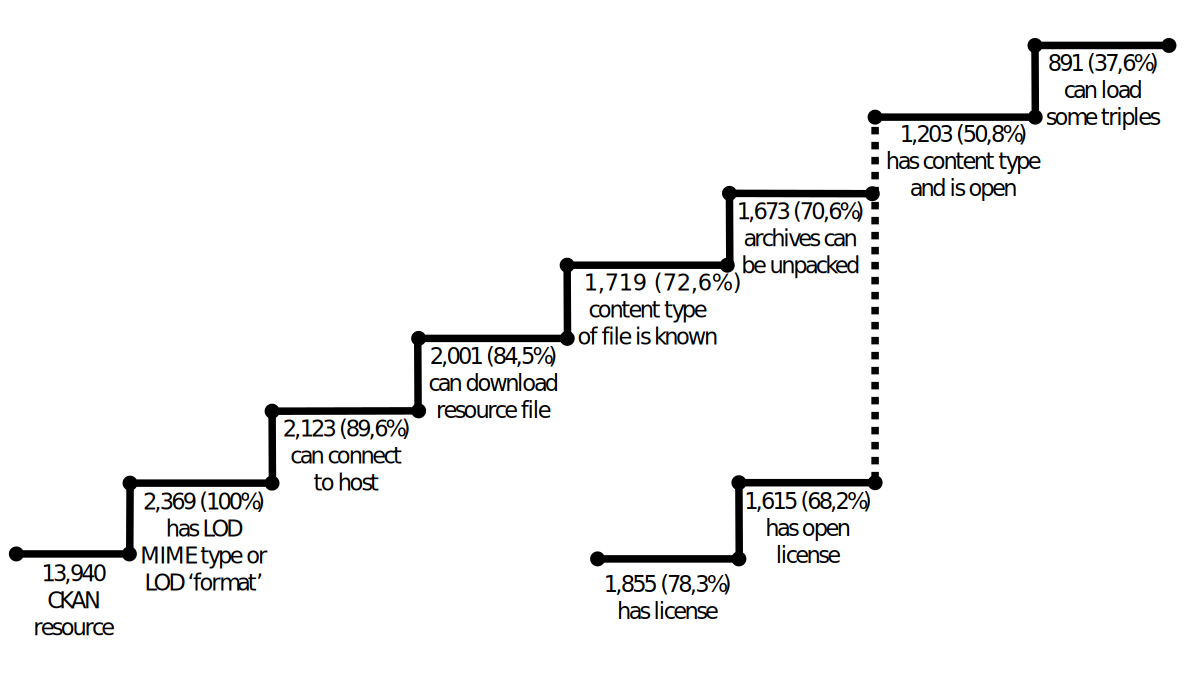
\includegraphics[width=0.9\textwidth]{./img/stairs}
  \caption{
    A `staircase' overview of the succes rates of the various tasks
     a machine agent has to perform in order to retrieve
     linked open data.
    The second stair from the left is the sample we have chosen to
     run our script on (set to 100\%);
     the percentages that appear in the other stairs are relative
     to this number.
    The stair in the top right corner shows that 37,6\% of
     the Datahub resources are fully machine-processable.
  }
\end{figure*}

%Maybe one or two diagram that show that success rates are conditional on
% e.g. domain (scientific versus governmental),
% sientific domain (medical versus rest),
% or ...

